Para esta demostración ocuparemos inducción fuerte. 

\textbf{BI}: Como el ciclo más pequeño es de largo 3 e impar, nuestro caso base se cumple, pues un grafo con un ciclo de largo 3 es isomorfo a $C_3$

\textbf{HI}: Supongamos que para un grafo con un ciclo de largo impar de tamaño $k$ < $n$, se cumple que este tiene un subgrafo inducido isomorfo a $C_3$ o $P_4$.

\textbf{TI}: Ahora pongamonos en dos casos. 

\begin{align*}
    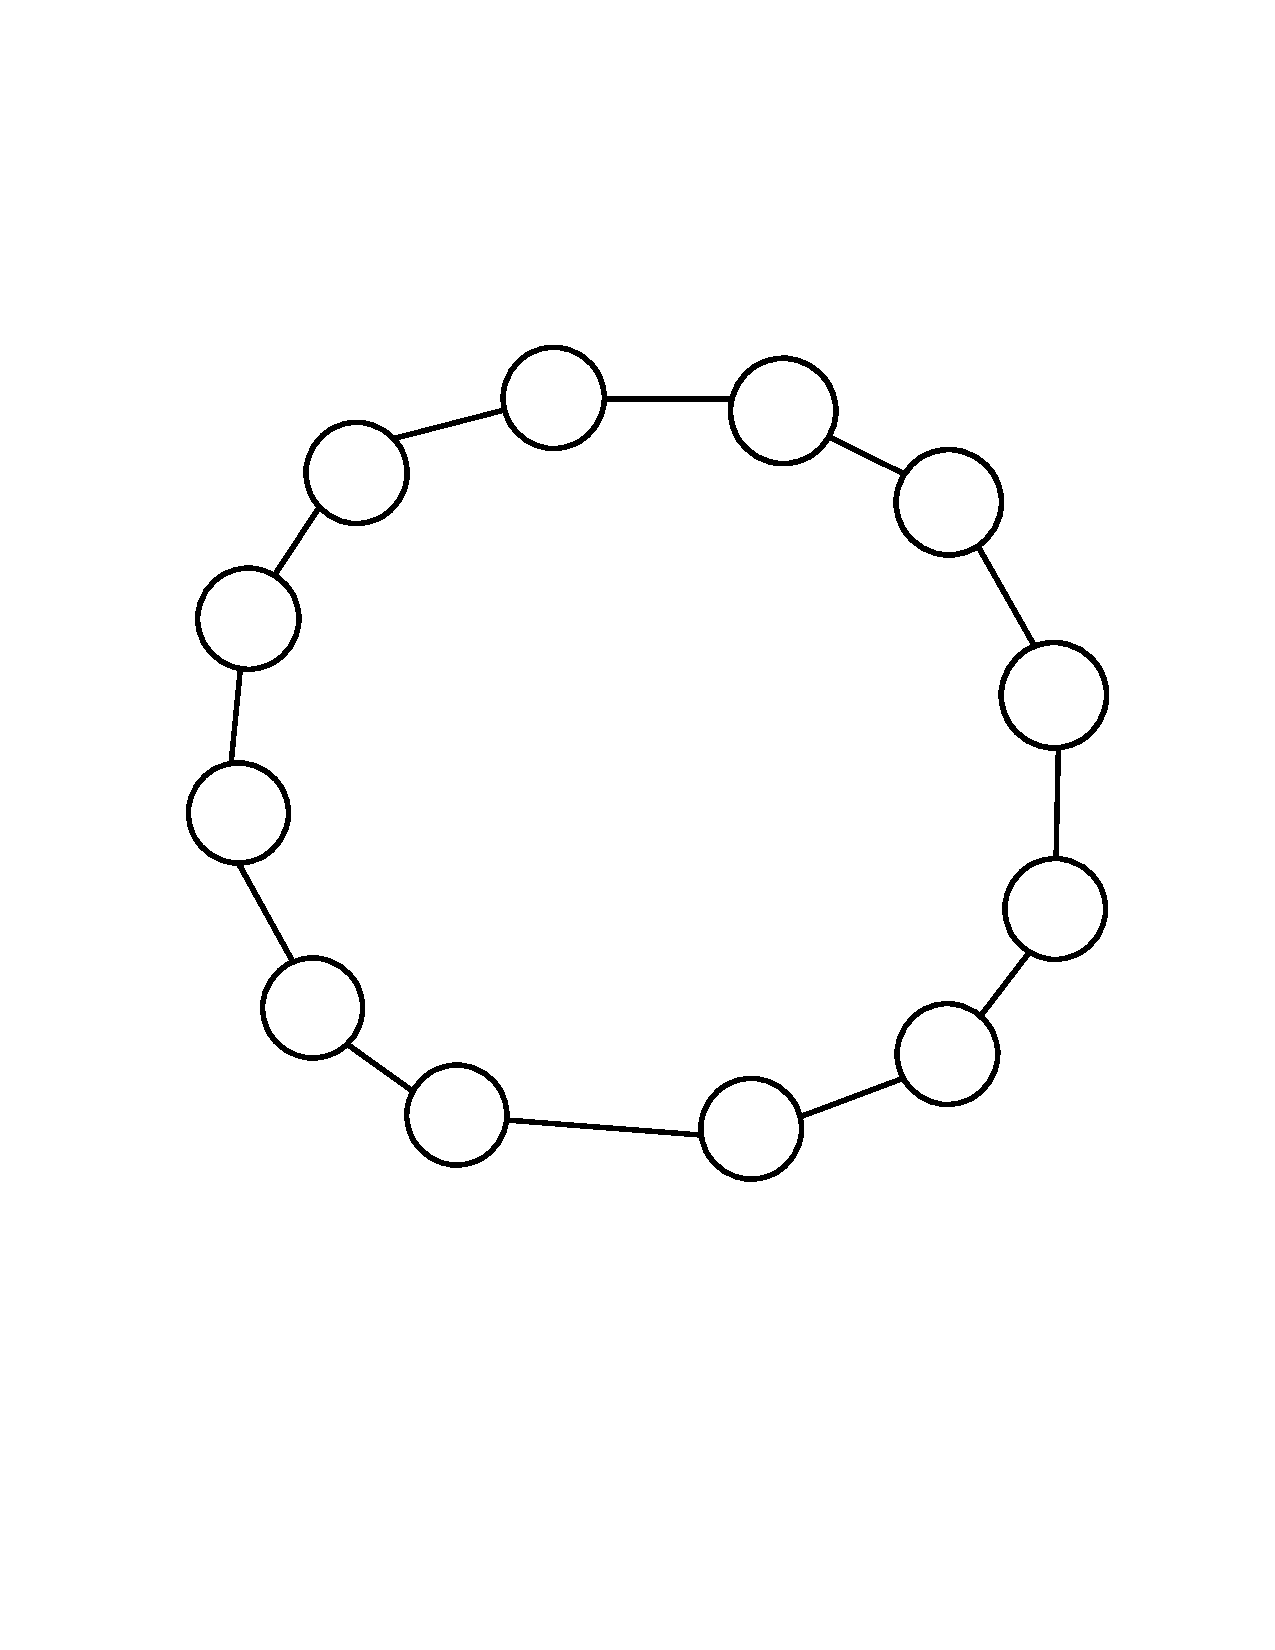
\includegraphics[width=6cm]{graph1.pdf}
\end{align*}

si tenemos un grafo con un ciclo de largo impar de tamaño $n$, y sin diagonales, claramente este tiene un subgrafo inducido isomorfo a $P_4$, pues es cosa de escoger 4 vertices cualesquiera y estos formaran un camino entre sus aristas. 

Si por el contrario nos encontramos con una diagonal 
\begin{align*}
    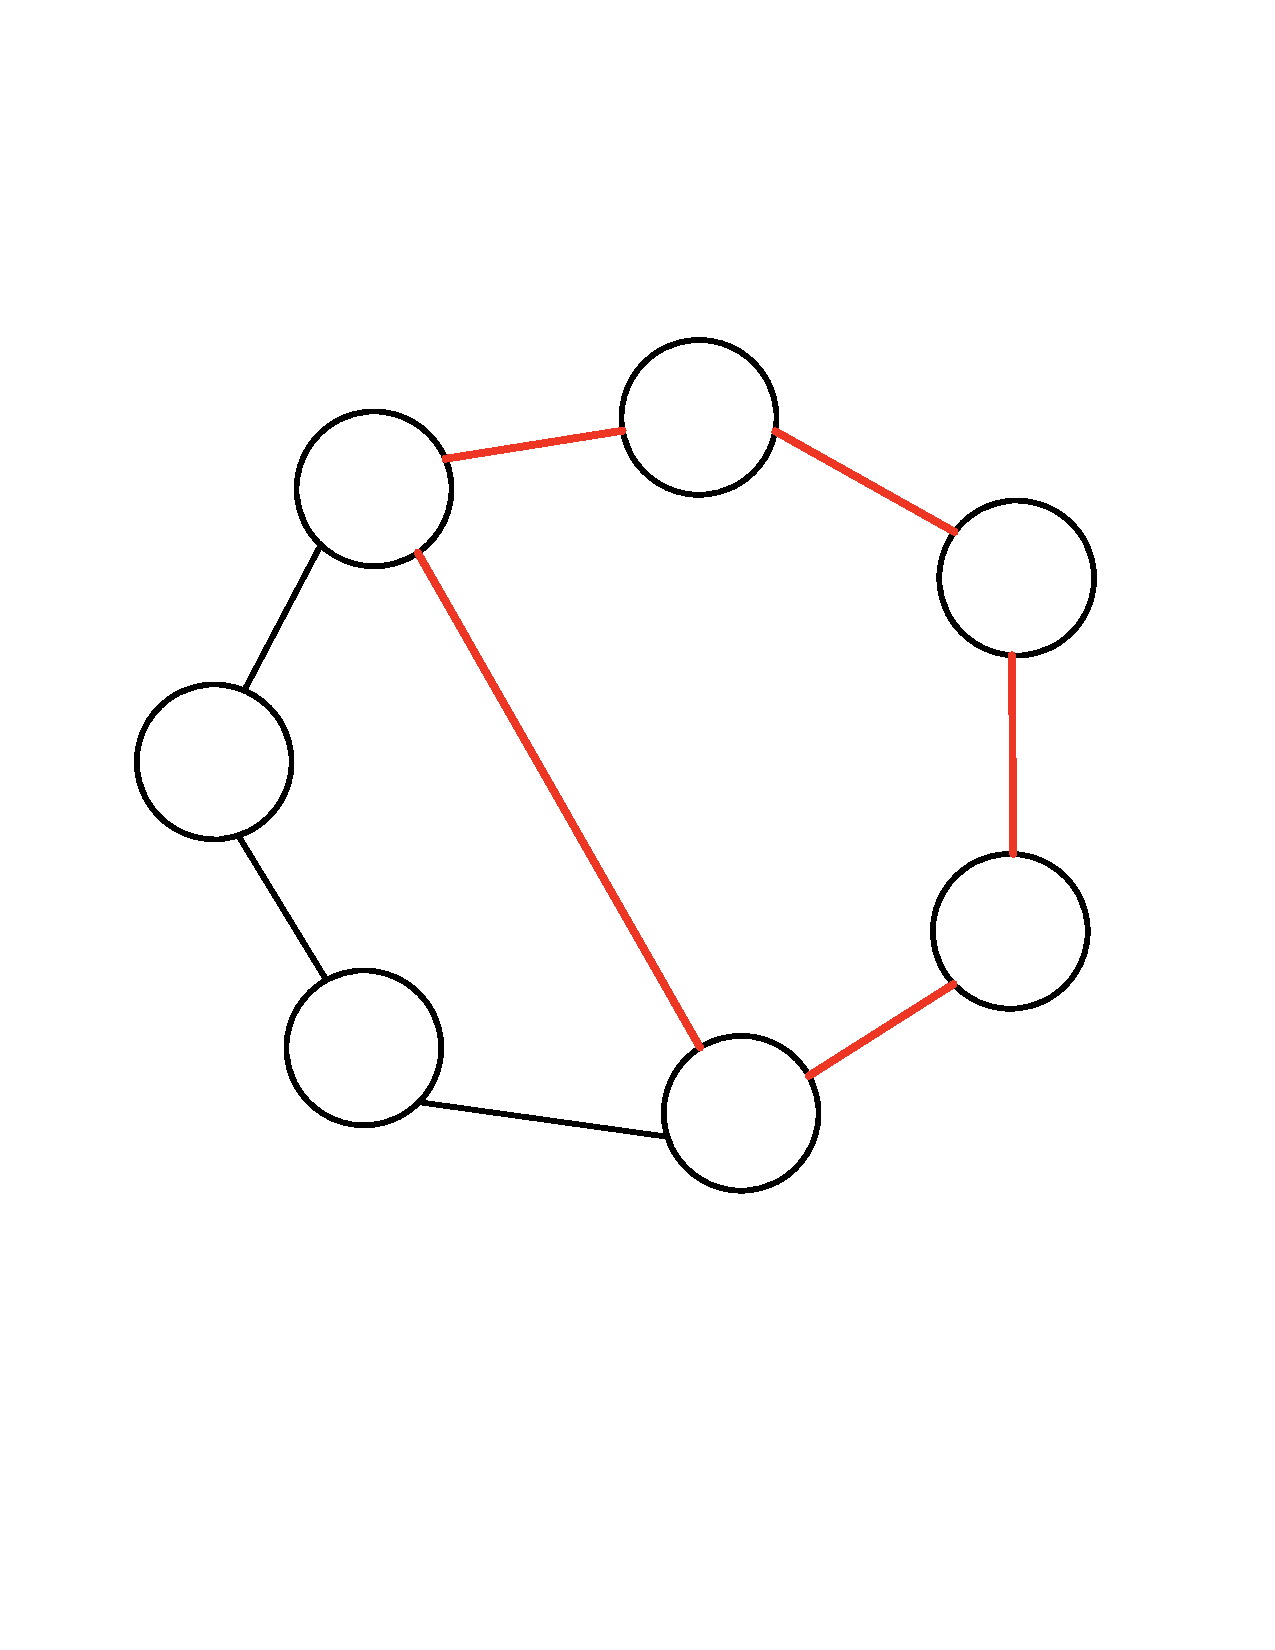
\includegraphics[width=6cm]{graph2.pdf}
\end{align*}
podemos separar el grafo en dos subgrafos, uno con número de aristas impares y otro con número de aristas pares. Resulta que el grafo con número aristas impares posee un ciclo de largo menor a $n$, y por hipótesis de inducción, cumple con tener un subgrafo inducido isomorfo a $C_3$ o $P_4$. Podemos aplicar esta lógica a cualquier grafo de manera recursiva, incluido un grafo completo, si este tiene un ciclo de largo impar, pues basta con ir dibujando las aristas una por una y fijandose en el grafo con número de aristas impares que se forma. De esta manera, queda demostrado que un grafo que posea un ciclo de largo impar, posee un subgrafo inducido isomorfo a $C_3$ o $P_4$.